\begin{frame}{Example: Step 1}
	$S = (OR_1, OR_2, OR_3)$, $OR_1 = ((b), (ph))$, $OR_2 = ((mt))$, $OR_2 = ((r))$
	
	\begin{figure}[h]
		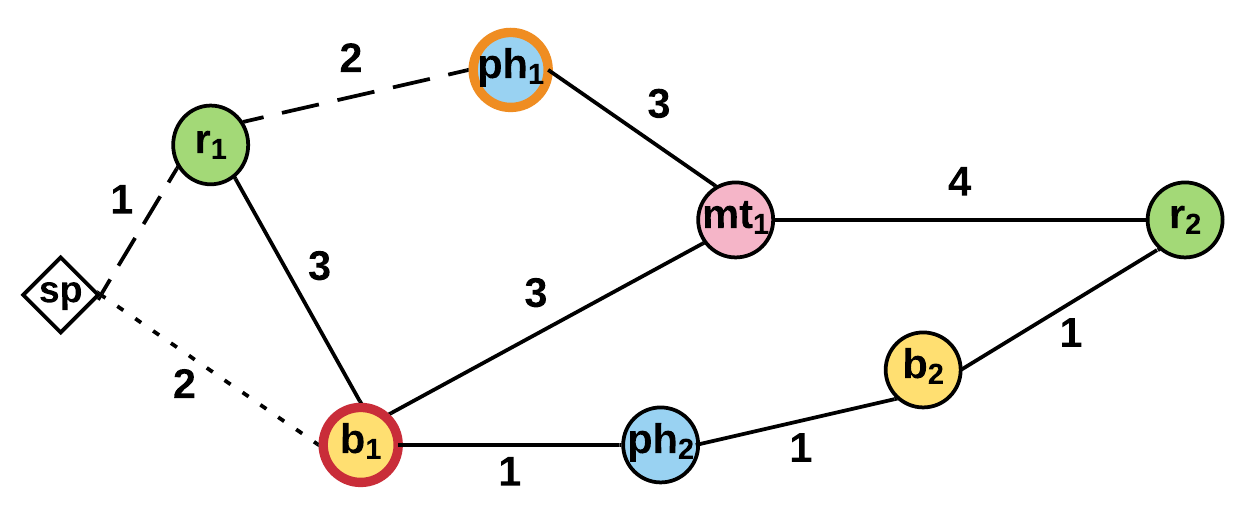
\includegraphics[scale=0.8]{Example_OR_1.png}
	\end{figure}
	
	\begin{table}[h]
		\centering
		\begin{tabular}{ |l|p{10cm}| } 
			\hline
			Step & Heap contents (PSR $R : length(r), index(R)$) \\
			\hline
			\textcolor{red}{1} & \textcolor{red}{$(b_1 : 2, 1)$} \\ 
			\hline
		\end{tabular}
	\end{table}

\end{frame}

\begin{frame}{Example: Step 2}
	$S = (OR_1, OR_2, OR_3)$, $OR_1 = ((b), (ph))$, $OR_2 = ((mt))$, $OR_2 = ((r))$
	
	\begin{figure}[h]
		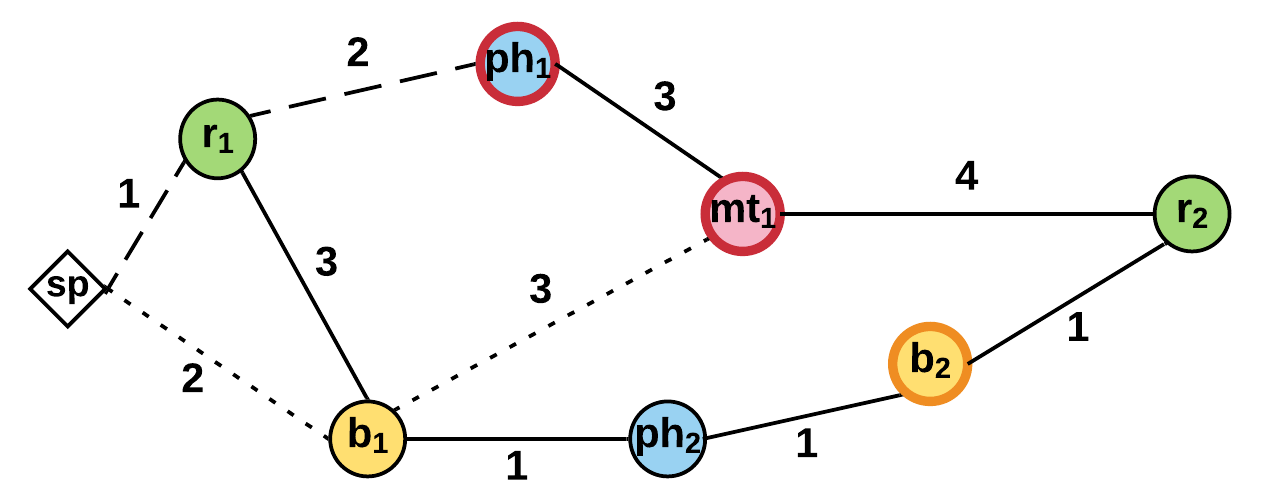
\includegraphics[scale=0.8]{Example_OR_2.png}
	\end{figure}
	
	\begin{table}[h]
		\centering
		\begin{tabular}{ |l|p{10cm}| } 
			\hline
			Step & Heap contents (PSR $R : length(r), index(R)$) \\
			\hline
			1 & $(b_1 : 2, 1)$ \\ 
			\hline
			\textcolor{red}{2} & \textcolor{red}{$(ph_1 : 3, 1)$}, \textcolor{red}{$(b_1, mt_1 : 5, 2)$} \\ 
			\hline
		\end{tabular}
	\end{table}

\end{frame}

\begin{frame}{Example: Step 6}
	$S = (OR_1, OR_2, OR_3)$, $OR_1 = ((b), (ph))$, $OR_2 = ((mt))$, $OR_2 = ((r))$
	
	\begin{figure}[h]
		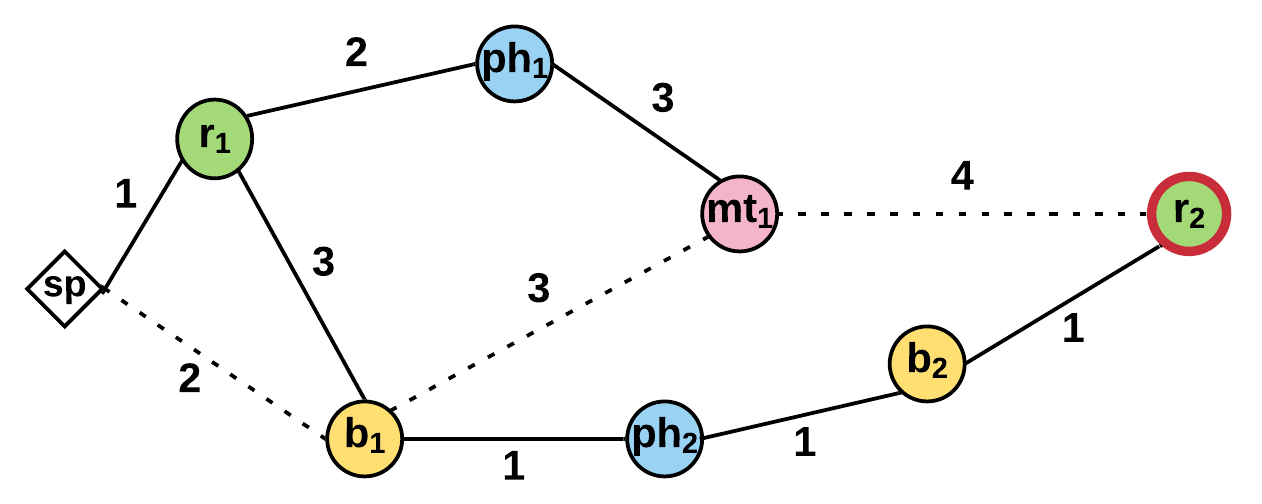
\includegraphics[scale=0.8]{Example_OR_6.png}
	\end{figure}
	
	\begin{table}[h]
		\centering
		\begin{tabular}{ |l|p{10cm}| } 
			\hline
			Step & Heap contents (PSR $R : length(r), index(R)$) \\
			\hline
			5 & $(b_1, mt_1 : 5, 2), (ph_1, mt_1 : 6, 2), (ph_2, mt_1 : 7, 2), (b_2, mt_1 : 9, 2)$ \\ 
			\hline
			\textcolor{red}{6} & $(ph_1, mt_1 : 6, 2), (ph_2, mt_1 : 7, 2), \textcolor{red}{(b_1, mt_1, r_2 : 9, 3)}, (b_2, mt_1 : 9, 2)$ \\ 
			\hline
		\end{tabular}
	\end{table}

\end{frame}

\begin{frame}{Example: Step 7}
	$S = (OR_1, OR_2, OR_3)$, $OR_1 = ((b), (ph))$, $OR_2 = ((mt))$, $OR_2 = ((r))$
	
	\begin{figure}[H]
		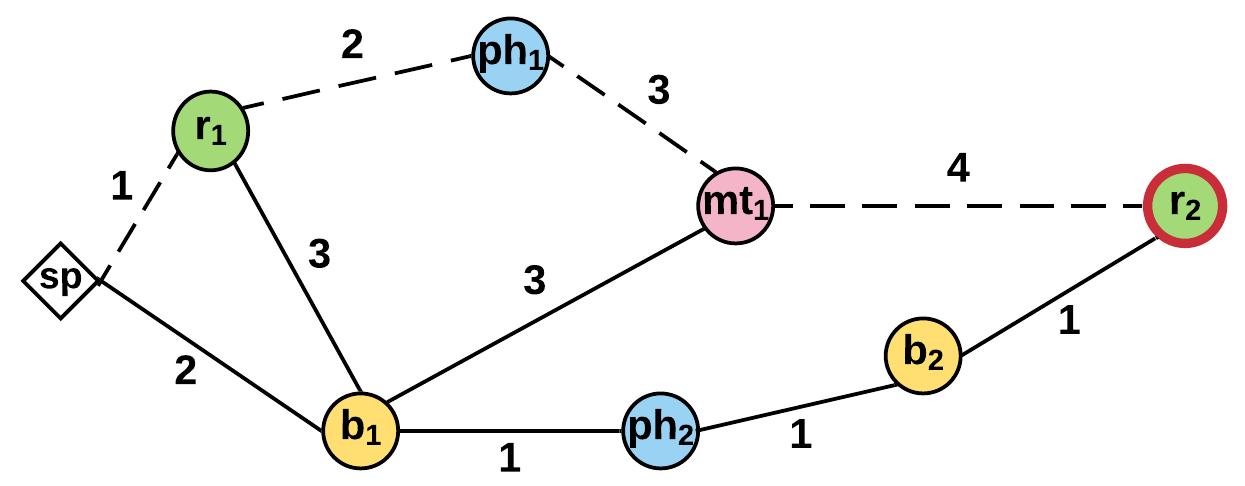
\includegraphics[scale=0.8]{Example_OR_7.png}
	\end{figure}
	
	\begin{table}[H]
		\centering
		\begin{tabular}{ |l|p{10cm}| } 
			\hline
			Step & Heap contents (PSR $R : length(r), index(R)$) \\
			\hline
			6 & $(ph_1, mt_1 : 6, 2), (ph_2, mt_1 : 7, 2), (b_1, mt_1, r_2 : 9, 3), (b_2, mt_1 : 9, 2)$ \\ 
			\hline
			\textcolor{red}{7} & $(ph_2, mt_1 : 7, 2), (b_1, mt_1, r_2 : 9, 3), (b_2, mt_1 : 9, 2),$ \textcolor{red}{\st{$(ph_1, mt_1, r_2 : 10, 3)$}} \\ 
			\hline
			8 & $(b_1, mt_1, r_2 : 9, 3), (b_2, mt_1 : 9, 2),$ \st{$(ph_2, mt_1, r_2 : 11, 3)$} \\ 
			\hline
		\end{tabular}
	\end{table}

\end{frame}

%\begin{frame}{Example}
%	\begin{table}[]
%		\centering
%		\begin{tabular}{ |l|p{10cm}| } 
%			\hline
%			Step & Heap contents (PSR $R : length(r), index(R)$) \\
%			\hline
%			1 & $(b_1 : 2, 1)$ \\ 
%			\hline
%			2 & $(ph_1 : 3, 1), (b_1, mt_1 : 5, 2)$ \\ 
%			\hline
%			3 & $(ph_2 : 3, 1), (ph_1, mt_1 : 6, 2), (b_1, mt_1 : 5, 2)$ \\ 
%			\hline
%			4 & $(b_2 : 4, 1), (b_1, mt_1 : 5, 2), (ph_1, mt_1 : 6, 2), (ph_2, mt_1 : 7, 2)$ \\ 
%			\hline
%			5 & $(b_1, mt_1 : 5, 2), (ph_1, mt_1 : 6, 2), (ph_2, mt_1 : 7, 2), (b_2, mt_1 : 9, 2)$ \\ 
%			\hline
%			6 & $(ph_1, mt_1 : 6, 2), (ph_2, mt_1 : 7, 2), (b_1, mt_1, r_2 : 9, 3), (b_2, mt_1 : 9, 2)$ \\ 
%			\hline
%			7 & $(ph_2, mt_1 : 7, 2), (b_1, mt_1, r_2 : 9, 3), (b_2, mt_1 : 9, 2),$ \st{$(ph_1, mt_1, r_2 : 10, 3)$} \\ 
%			\hline
%			8 & $(b_1, mt_1, r_2 : 9, 3), (b_2, mt_1 : 9, 2),$ \st{$(ph_2, mt_1, r_2 : 11, 3)$} \\ 
%			\hline
%		\end{tabular}
%	\end{table}
%\end{frame}